\documentclass[aspectratio=43]{beamer}
\usetheme{Boadilla}
\usepackage{duarteBeamer}
% \usepackage{lighttheme}

% ----------------------------

% ============================
% DADOS
\title[ANN para Detecção de Danos em Trilhos]{Redes Neurais Artificiais para Detecção de Danos em Trilhos}
\author[Gabriel D. Silva]{
	% \raggedright
	\begin{tabular}{ll}
	Gabriel D. Silva & {} \\ 
	{\footnotesize gd.silva@unesp.br} & {}
	\end{tabular}
}
\institute[FEIS/UNESP]{Universidade Estadual Paulista \\ Departamento de Engenaria Mecânica \\ Área de Mecânica dos Sólidos e Projetos \\ Grupo de Sistemas e Materiais Inteligentes}
% \logo{
\includegraphics[scale=0.02]{figures/logos/unesp_ilha.pdf}}
\date{12 de maio de 2023}
% ----------------------------

\begin{document}
% ============================
% CAPA E SUMÁRIO
{%\setbeamertemplate{footline}{}
\begin{frame}
	\titlepage
\end{frame}
}
% \begin{frame}{Sumário}
% 	\tableofcontents
% \end{frame}
% ----------------------------

% ============================
% SEÇÕES
\chapter{Literature Review}\label{sec:literature_review}

This chapter deals with the history, the main concepts and some practical cases of \gls*{shm} inside the industry and academic area, besides showing how it may be used in the railway crack detection context.
Next, in the dynamic field, it will be studied the main mechanical concepts to get the necessary understanding to an \gls*{uav} motion as well the basics to know how an \gls*{uav} can be controlled.
Then, it will be shown the mathematics behind the algorithms of deep learning that will be implemented in the \cref{sec:results}. 
Finally, the way how the algorithms are going to be implemented and the tools necessary to achieve the desired \gls*{nn}.
\section{Metodologia}

\begin{frame}{Sistema Inteligente}

    \[\boxed{\text{\alert<2>{Inteligência artificial}} + \text{Engenharia} = \text{Sistema Inteligente}}\] 
\end{frame}

\begin{frame}{Redes Neurais (Artificiais)}
\pause
\begin{figure}
\centering
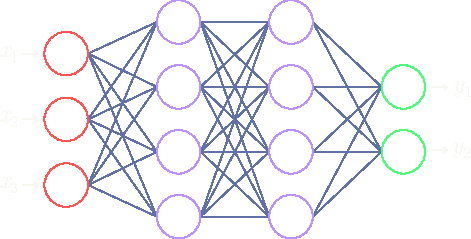
\includegraphics{figures/rede_neural.pdf}
\end{figure}
\pause
\begin{table}
\centering
\begin{tabular}{|l|l|l|}
    \hline
    Caso & \(x_i\)           & \(y_i\)             \\ \hline
    SHM  & dados PZT         & \alert<4>{problemas no trilho} \\ \hline
    VANT & \(S_0\) e \(S_i\) & forças atuantes     \\ \hline
\end{tabular}
\end{table}
\end{frame}

\begin{frame}{Implementação}
\pause
\begin{itemize}
    \item \textbf{SHM}
        \begin{itemize}
            \item<3-4> Utilização do algoritmo já disponível.
            \item<3-4> MATLAB para geração de dados.
            \item<3-4> PyTorch para modelagem da rede neural.
        \end{itemize}
    \item \textbf{VANT}
    \begin{itemize}
        \item<4> Dados fornecidos pela VALE.
        \item<4> PyTorch para modelagem da rede neural.
    \end{itemize}
\end{itemize}
    
\end{frame}
\section{Conclusão}

% ===========================
\begin{frame}{Desafios}
\begin{itemize}
    \item Desenvolvimento da rede neural.
    \item Determinar qual rede neural é a mais adequada.
    \item Definir a forma da aquisição de dados.
    \begin{itemize}
        \item Definir a rede neural.
        \item Otimizar a rede neural
    \end{itemize}
\end{itemize}

\begin{block}{Trabalhos Posteriores}
    \begin{itemize}
        \item Desenvolver o algoritmo no \matlab sem a interface gráfica.
        \item Migrar o algoritmo para frameworks específicos de deep learning (TensorFlow, PyTotrch, etc)
    \end{itemize}
\end{block}
\end{frame}
% ----------------------------
\end{document}